%%%%%%%%%%%%%%%%%%%%%%%%%%%%%%%%%%%%%%%%%
% Beamer Presentation
% LaTeX Template
% Version 1.0 (10/11/12)
%
% This template has been downloaded from:
% http://www.LaTeXTemplates.com
%
% License:
% CC BY-NC-SA 3.0 (http://creativecommons.org/licenses/by-nc-sa/3.0/)
%
%%%%%%%%%%%%%%%%%%%%%%%%%%%%%%%%%%%%%%%%%

%----------------------------------------------------------------------------------------
%	PACKAGES AND THEMES
%----------------------------------------------------------------------------------------

\documentclass{beamer}

\mode<presentation> {
	
	% The Beamer class comes with a number of default slide themes
	% which change the colors and layouts of slides. Below this is a list
	% of all the themes, uncomment each in turn to see what they look like.
	
	%\usetheme{default}
	\usetheme{AnnArbor}
	%\usetheme{Antibes}
	%\usetheme{Bergen}
	%\usetheme{Berkeley}
	%\usetheme{Berlin}
	%\usetheme{Boadilla}
	%\usetheme{CambridgeUS}
	%\usetheme{Copenhagen}
	%\usetheme{Darmstadt}
	%\usetheme{Dresden}
	%\usetheme{Frankfurt}
	%\usetheme{Goettingen}
	%\usetheme{Hannover}
	%\usetheme{Ilmenau}
	%\usetheme{JuanLesPins}
	%\usetheme{Luebeck}
	%\usetheme{Madrid}
	%\usetheme{Malmoe}
	%\usetheme{Marburg}
	%\usetheme{Montpellier}
	%\usetheme{PaloAlto}
	%\usetheme{Pittsburgh}
	%\usetheme{Rochester}
	%\usetheme{Singapore}
	%\usetheme{Szeged}
	%\usetheme{Warsaw}
	
	% As well as themes, the Beamer class has a number of color themes
	% for any slide theme. Uncomment each of these in turn to see how it
	% changes the colors of your current slide theme.
	
	%\usecolortheme{albatross}
	\usecolortheme{beaver}
	%\usecolortheme{beetle}
	%\usecolortheme{crane}
	%\usecolortheme{dolphin}
	%\usecolortheme{dove}
	%\usecolortheme{fly}
	%\usecolortheme{lily}
	%\usecolortheme{orchid}
	%\usecolortheme{rose}
	%\usecolortheme{seagull}
	%\usecolortheme{seahorse}
	%\usecolortheme{whale}
	%\usecolortheme{wolverine}
	
	%\setbeamertemplate{footline} % To remove the footer line in all slides uncomment this line
	%\setbeamertemplate{footline}[page number] % To replace the footer line in all slides with a simple slide count uncomment this line
	
	%\setbeamertemplate{navigation symbols}{} % To remove the navigation symbols from the bottom of all slides uncomment this line
}

\usepackage{graphicx} % Allows including images
\usepackage{booktabs} % Allows the use of \toprule, \midrule and \bottomrule in tables
%\usepackage{movie15}
%%%%% SPECIAL PACKAGES %%%%%%%%%%
\usepackage{setspace}
%\usepackage[ngerman]{babel}
\usepackage[utf8]{inputenc}
\usepackage{fancyhdr}
\usepackage{tabularx}
%\renewcommand{\rmdefault}{phv}
%\renewcommand{\sfdefault}{phv}

\setcounter{tocdepth}{2} % to get subsubsections in toc 
% cf. http://www.latex-community.org/forum/viewtopic.php?f=47&p=44760

\usepackage{amssymb,latexsym}
\usepackage{amsmath, amsthm}
\usepackage{mathabx}

%for bibliography; installation using 'sudo tlmgr install amsrefs'
%\usepackage{amsrefs}

\usepackage{graphics}
\usepackage{animate}
%\usepackage{xmpmulti}

\usepackage{hyperref}
\hypersetup{colorlinks=true, urlcolor=blue}
\usepackage{hyperref}

\usepackage{cancel} % http://jansoehlke.com/2010/06/strikethrough-in-latex/

%\usepackage{listings} %
% http://en.wikibooks.org/wiki/LaTeX/Source_Code_Listings
% http://olmjo.com/files/teaching/PSC505/LaTeXandR.pdf
\usepackage[natbib=true,style=authoryear,backend=bibtex,useprefix=true]{biblatex}
\addbibresource{main.bib}


% package for flower symbol (\ding(96))
\usepackage{pifont}
% required installation: sudo apt-get install texlive-fonts-recommended (30MB)
% http://tug.ctan.org/info/symbols/comprehensive/symbols-a4.pdf

\usepackage{tikz} % for diagrams
\usetikzlibrary{matrix,positioning,arrows,calc,decorations.pathmorphing,shapes}
% for snaky lines (http://tex.stackexchange.com/questions/209942/curved-arrows-in-tikz) 
\tikzset{snake it/.style={-stealth,
		decoration={snake, 
			amplitude = .4mm,
			segment length = 2mm,
			post length=0.9mm},decorate}}

\usepackage[parfill]{parskip}

\usepackage{framed} %for putting some text in boxes using \begin{framed}
	
	\usepackage{enumerate}
	
	%for displaying tensor indices properly. requires installation of tensor package using 'sudo tlmgr install tensor'
	\usepackage{tensor}
	
	%for placing captions of figures on the side instead of above/below the figure
	\usepackage{sidecap}
	\linespread{1.2}
	
	%plain makes sure that we have page numbers
	%\pagestyle{plain}
	
	\theoremstyle{plain}
	\newtheorem{axiom}{Axiom}
	\newtheorem*{main}{Main Theorem}
	\newtheorem{proposition}{Proposition}
	
	\theoremstyle{definition}
	
	\theoremstyle{remark}
	\newtheorem*{notation}{Notation}
	
	\numberwithin{equation}{section}
	\numberwithin{figure}{section}
	\numberwithin{theorem}{section}
	\usepackage{bibentry}
	
	%symbol for maps
	\renewcommand{\to}{\longrightarrow}
	\newcommand{\injmapto}{\hookrightarrow}
	\newcommand{\surjmapto}{\twoheadrightarrow}
	\newcommand{\linearmapto}{\stackrel{\sim}{\longrightarrow}}
	\newcommand{\projmapto}{\stackrel{\pi}{\longrightarrow}}
	
	%for real numbers
	\newcommand{\R}{\mathbb{R}}
	
	% manifold, atlas and topology
	\newcommand{\A}{\mathcal{A}}
	%\newcommand{\O}{\mathcal{O}}
	\newcommand{\mfd}{(M, \mathcal{O}, \mathcal{A})}
	
	\newcommand{\after}{\circ}
	\newcommand{\stdtop}{\mathcal{O}_{std}}
	\newcommand{\cibasis}[2][]{\frac{\partial #1}{\partial #2}}
	
	%connection coefficient functions or gammas
	\newcommand{\ccf}[2]{\Gamma\indices{^{#1}_{#2}}}
	\newcommand{\ccfx}[3]{\left(\Gamma_{#3}\right)\indices{^{#1}_{#2}}} % with chart index
	
	%set theory symbols
	%\renewcommand{\exists}{\exists\,}
	%\renewcommand{\forall}{\forall\,}
	
	%This defines a new command \questionhead which takes one argument and prints out Question #. with some space.
	\newcommand{\questionhead}[1]
	{
		\noindent{\small\bf Question #1.}
	}
	
	\newcommand{\problemhead}[1]
	{
		\noindent{\small\bf Problem #1.}
	}
	
	\newcommand{\exercisehead}[1]
	{ \smallskip
		\noindent{\small\bf Exercise #1.}
	}
	
	\newcommand{\solutionhead}[1]
	{
		\noindent{\small\bf Solution #1.}
	}
	
	\newcommand{\bubblethis}[2]{
		\tikz[remember picture,baseline]{\node[anchor=base,inner sep=0,outer sep=0](#1) {#1};\node[overlay,cloud callout,callout relative pointer={(0.2cm,-0.7cm)}, aspect=2.5,fill=white!90] at ($(#1.north)+(-0.5cm,1.6cm)$) {#2};}
	}
	
	\setbeamertemplate{sidebar right}{}% or get rid of navigation entries there somehow
	\addtobeamertemplate{footline}{\hfill\usebeamertemplate***{navigation symbols}%
		\hspace*{0.1cm}\par\vskip 2pt}{}
	%\setbeamertemplate{footnote}{%
	%	\hangpara{2em}{1}%
	%	\makebox[2em][l]{\insertfootnotemark}\footnotesize\insertfootnotetext\par%
	%}	
%%%%%%%%%%%%%%%%%%%%%%%%%%%%%
	
	
	%----------------------------------------------------------------------------------------
	%	TITLE PAGE
	%----------------------------------------------------------------------------------------
	\title[Topics in Physics]{Topics in Physics} % The short title appears at the bottom of every slide, the full title is only on the title page
	
	\author{Piyush Kaul } % Your name
	\institute[https://piyushkaul.github.io] % Your institution as it will appear on the bottom of every slide, may be shorthand to save space
	{
		\\ % Your institution for the title page
		\medskip
		\textit{piyushkaul@ieee.org} % Your email address
	}
	\date{\today} % Date, can be changed to a custom date
	
	\begin{document}
		
		\begin{frame}
			\titlepage % Print the title page as the first slide
		\end{frame}
		
		\begin{frame}
			\frametitle{Overview} % Table of contents slide, comment this block out to remove it
			\tableofcontents % Throughout your presentation, if you choose to use \section{} and \subsection{} commands, these will automatically be printed on this slide as an overview of your presentation
		\end{frame}
		
		%----------------------------------------------------------------------------------------
		%	PRESENTATION SLIDES
		%----------------------------------------------------------------------------------------
		
		%------------------------------------------------
		\section{Special Theory of Relativity} % Sections can be created in order to organize your presentation into discrete blocks, all sections and subsections are automatically printed in the table of contents as an overview of the talk
		%------------------------------------------------
		
		
		\begin{frame}[shrink]
			\frametitle{Relativity}
			Objective
			\begin{enumerate}
				\item Special Theory of Relativity: Einstein published in 1905 (annus mirablis). Concerns inertial frames of reference. No gravity.
				\item General Theory of Relativity. Einstein publushed in 1915. Concerns non-inertialframes. Gravity incorporated.
			\end{enumerate}
			\begin{definition}Principle of Relativity:\\
				The motion of bodies included in a given space are same among themselves, whether that space is at or rest or moves uniformly in a straight line.			\footnote[frame]{\cite{feynman1965}}
			\end{definition}
			\begin{example}
				If a spaceship is drifting along a uniform speed, all experiments performed in the spaceship and all phenomena in spaceship will appear same as if spaceship is not moving at all. There is no way to find out that spaceship is moving without looking outside.
			\end{example}
		\end{frame}
	
		\begin{frame}[shrink]
			\begin{figure}\footnotemark[1]
				\centering
				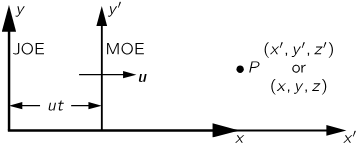
\includegraphics[width=0.7\linewidth]{figures/screenshot001}
				\caption[Two Co-ordinate systems in relative motion]{Two Co-ordinate systems in relative motion}
				\label{fig:screenshot001}
			\end{figure}
			\footnotetext[1]{\cite{feynman1965feynman}}
			Let Moe be moving in direction x with uniform speed u.
			Then 
			\begin{align}
				& x' = x - ut \\
				& y' = y \\
				& z' = z \\
				& t' = t
			\end{align}
		\end{frame}
		
		
		\begin{frame}[shrink]
			\frametitle{Simultaneity}
		If we substitute the previous co-ordinate transformation in Newtons laws of Mechanics, the laws stay the same. So it is impossible to tell whether we are in moving or stationary state.
		
		However Maxwell equations don't conform to the same.
		
		Maxwell equations expect the speed of light to be independent of movement of source. Also the speed of light goes out at same speed of c in all directions.
		
		However, Maxwell’s Equations of electromagnetism predict an electromagnetic radiation moving through space in any direction at exactly the speed of light.
		
		This is, or appears to be, in conflict with Galilean invariance ,and suggests that by examining electricity and magnetism, rather than just mechanics, it is possible to determine who is ‘at rest’ in the Universe. It would be the person who measures lightspeed as exactly the same in every single direction through space.\footnotemark[2]
		
		The Michelson-Morley experiment showed, on the contrary, that an observer A (on Earth in January) and observer B (on Earth in July) moving through space relative to each other will both measure lightspeed uniform and the same in all directions.
		
		So both Galilean invariance and uniform lightspeed turn out to be true. Einstein coped with it by developing the weird spacetime of Special Relativity.
		\footnotetext{\url{https://www.quora.com/What-is-the-conflict-between-Newtons-law-of-motion-and-Maxwell-s-theory-of-electromagnetism}}
		
		\end{frame}
		
		\begin{frame}
			\frametitle{LoRA - Results}
			\begin{enumerate}
				\item Reduce memory size by 1000 times. 350 GB $\to$ 35 MB
			\end{enumerate}
		\end{frame}
		
		
		
		
		\section{Quantum Mechanics}
		\begin{frame}
			\frametitle{QLoRA: Efficient Fine-tuning of Quantized LLM}
			QLoRA reduces memory requirement from $>$ 700 GB of GPU to $<$48 GB
			Following advantages are mentioned
			\begin{enumerate}
				\item 4-bit Normal Float. Better than 4-bit integer and 4-bit float
				\item Double Quantization. Quantizing Quant info (saving of approx 3GB for 65 GB)
				\item Paged Optimizers. Avoid gradient check pointing spikes.
			\end{enumerate}
		\end{frame}
		
		\begin{frame}[shrink]
			\frametitle{QLoRA: 4-bit Normal Float}
			\begin{enumerate}
				\item Storage as 4b NF. Convert to BF16 for usage.
				\item The main limitation of quantile quantization is estimating quantiles.
				\item We fix the datatype range [-1,1]. The quantiles of datatype and NN weights need to be matched
				\item Estimate $2^{k+1}$ quantiles for $N(0,1)$ to obtain k-bit quantile regression
				\item Normalize its values in [-1, 1] range
				\item Quantize input by Re scaling to [-1,1] range
			\end{enumerate}                        
			
			\begin{align}
				q_i = \frac{1}{2} (Qx(\frac{i}{2^k+1}) + Qx(\frac{i+1}{2^k+1})    
			\end{align}
			To solve the problem or representing zero exactly, we do this separately for +ve and -ve range.
		\end{frame}                        
		
		
		\section{Riemannian Geometry}
		\begin{frame}
			\frametitle{ZeroQuant-FP}
			Contribution
			\begin{enumerate}
				\item Negligible degradation from FP16 to FP8
				\item FP8 activation along with FP4 weights. LoRC compensates quantization error for w4a8
				\item FP4 weights need to be converted to FP8 for inference. Can be done dynamically. 
				\item Complexity reduction by having scale factors only in power of 2
			\end{enumerate}
		\end{frame}
		

		
		
		\begin{frame}
			\frametitle{Quantum Computing}
			\begin{enumerate}
				\item Input to q-proj is Normal
				\item The output of q-proj and FC are skewed
				\item Integer quantization is not ideal to process skewness
				\begin{align}
					Q(x) = INT(X- Z/S) - Z
				\end{align}
				\item Integer quantization not ideal for outliers.
			\end{enumerate}
		\end{frame}
		

		\begin{frame}
			\frametitle{Techniques Used}
			\begin{enumerate}
				\item Zero Quant V2 (FGQ and Token Wise Quantization)
				\item LoRC
				\item Casting FP8 to FP4 with restricted scale
			\end{enumerate}
			Two methods used for restricting the scale
			\begin{enumerate}
				\item Map to nearest values represented by power of t2 i.e. $\hat{S} = 2^{log_2(S)}$
				\item Collect scale in vector $s= [S_1,.. S_x]$. Take maximum and denote by $S_{max}$. Adjust  $S_{max}/s$
			\end{enumerate}
		\end{frame}
		
		
		
		

		\begin{frame}
			\frametitle{ZeroQuant-FP}
			Contribution
			\begin{enumerate}
				\item Negligible degradation from FP16 to FP8
				\item FP8 activation along with FP4 weights. LoRC compensates quantization error for w4a8
				\item FP4 weights need to be converted to FP8 for inference. Can be done dynamically. 
				\item Complexity reduction by having scale factors only in power of 2
			\end{enumerate}
		\end{frame}
		
		
\section{General Theory of Relativity - Graviation}
\begin{frame}
	\frametitle{ZeroQuant-FP}
	Contribution
	\begin{enumerate}
		\item Negligible degradation from FP16 to FP8
		\item FP8 activation along with FP4 weights. LoRC compensates quantization error for w4a8
		\item FP4 weights need to be converted to FP8 for inference. Can be done dynamically. 
		\item Complexity reduction by having scale factors only in power of 2
	\end{enumerate}
\end{frame}

		\section{Quantum Computing}
		
		
		%\begin{frame}
		%\frametitle {Zero Quant V2: Sensitivity Analysis}
		%\begin{enumerate}
		%\item INT8 weight-only quantization can serve as a standard
		%method for reducing memory costs in LLMs, with negligible degradation in accuracy.
		%\item INT4
		%weight-only quantization for small models results in substantial accuracy degradation (Class-3), but
		%this effect lessens as the model size increases (Class-2)
		%\item Contrary to (2), INT8 activation results in
		%minimal accuracy drops for small models (Class-1) but larger models exhibit greater drops (Class-3).
		%\item  With INT8 activation, BLOOM shows no divergence issues up to a model size of 176B, whereas
		%OPT performs poorly from ≥ 6.7B model sizes.
		%\end{enumerate}
		%\end{frame}
		
		
		
		%------------------------------------------------
		
\begin{frame}[allowframebreaks, noframenumbering]
	\frametitle{Bibliography}
	\printbibliography
	\nocite{*}
\end{frame}

		
		%------------------------------------------------
		
		\begin{frame}
			\Huge{\centerline{The End}}
		\end{frame}
		
		%----------------------------------------------------------------------------------------
		

@book{feyn1,
	author = {Richard Feynman},
	title = {Feynman's Lectures in Physics},
	date = {1970},
}
	\end{document} 